%% STM32 Industrial Controller Datasheet
%% Customized for DarcyJProjects

\documentclass[10pt]{datasheet}

% Standard packages
\usepackage[utf8]{inputenc}
\usepackage[english]{babel}
\usepackage{graphicx} % Needed for inserting photos/block diagrams
\usepackage{tabularx} % Better tables
\usepackage{float} % Keep things where they should be
\usepackage{enumitem}
% Allows absolute positioning of text (for the version stamp)
\usepackage[absolute]{textpos}


% Document Meta-Data
\title{STM32G4 Embedded Industrial Controller}
\author{DarcyJProjects}
\date{February 2026}
\revision{Rev 1.0}
\companylogo{
    % Negative value (-0.2\height) pushes the image DOWN by 20% of its own height
    \raisebox{-0.22\height}{
\includegraphics[width=1cm]{cropped-logo-5-300x300.png}}
    \hspace{0cm} % Adds a small gap between logo and text
    \Huge \textbf{DarcyJProjects}
} % Simple text logo for now

\begin{document}

% --- HARDWARE VERSION STAMP ---
% {5cm} is the width of the box
% (15cm, 1cm) are the X, Y coordinates from the top-left of the page
% Adjust 15cm to move it Left/Right, Adjust 1cm to move it Up/Down
\begin{textblock*}{5cm}(15cm, 2.5cm) 
    \raggedleft % Align text to the right
    \small 
    \textbf{Hardware Ver:} v1.XXX
\end{textblock*}

\maketitle

\section{Features}
\begin{itemize}[leftmargin=*, itemsep=2pt, topsep=0pt]
    \item \textbf{Core:} STM32G431 Cortex-M4 MCU @ 170MHz
    \item \textbf{Power:} 7V-28V DC (Rev. Polarity, OCP, TVS)
    \item \textbf{Isolation \& Protection:} 1 kV Galvanic Isolation, ESD Protection up to 30 kV
    
    % CONDENSING STRATEGY: Use a paragraph style for the big lists.
    % Notice how we just list them with commas instead of new bullets.
    \item \textbf{Field I/O (All Isolated):}
    4x Analog Inputs (12-bit, 4-20mA/0-5V),
    2x Analog Outputs (12-bit, 4-20mA/0-5V),
    4x Digital Inputs (24V),
    2x Digital Outputs (24V),
    2x Relays (10A / 30VDC, 50VAC),
    Isolated $I^2$C Header.

    \item \textbf{On-Board HMI:} 
    0.96" OLED Display, 
    4x Tactile Buttons, 
    5x Status LEDs, 
    6x Hardware Mode Switches (Analog Current/Voltage Mode Config).

    \item \textbf{Memory:} 4KB EEPROM with CRC (Stores Config \& Automation Rules)

    \item \textbf{Connectivity:}
    Isolated RS485 (MODBUS RTU Master/Slave);
    USB-C (DFU Flashing \& Serial Debug)

    \item \textbf{Reliability:} 4-Layer PCB with Isolation Barrier, PPTC Fuses, TVS Protection.
    \item \textbf{Control:} Web Panel with custom "No-Code" automation engine; Full MODBUS RTU support for SCADA integration.
\end{itemize}







\section{Intended Applications}
\begin{itemize}[leftmargin=*, itemsep=2pt, topsep=0pt]
    \item \textbf{Industrial Sensor Node:} Aggregation of 4-20mA process signals (pressure, flow, level) to MODBUS RTU.
    \item \textbf{Distributed I/O Expansion:} Cost-effective relay control and status monitoring for existing SCADA networks.
    \item \textbf{Hybrid Edge Controller:} Autonomous control of downstream MODBUS slaves (e.g., VFDs, remote sensors) while simultaneously reporting status to an upstream SCADA system.
    \item \textbf{Embedded Logic Prototyping:} Development platform for custom control loops and automation logic using the STM32G4.
\end{itemize}

% --- SECTION 3: VISUALS ---
% \vfill\break % Force column break so images sit nicely on the right

\begin{figure}[h]
    \centering
    % REPLACE 'example-image' with your actual filename (e.g., board_photo.png)
    % You can upload files to Overleaf using the upload button on the left.
    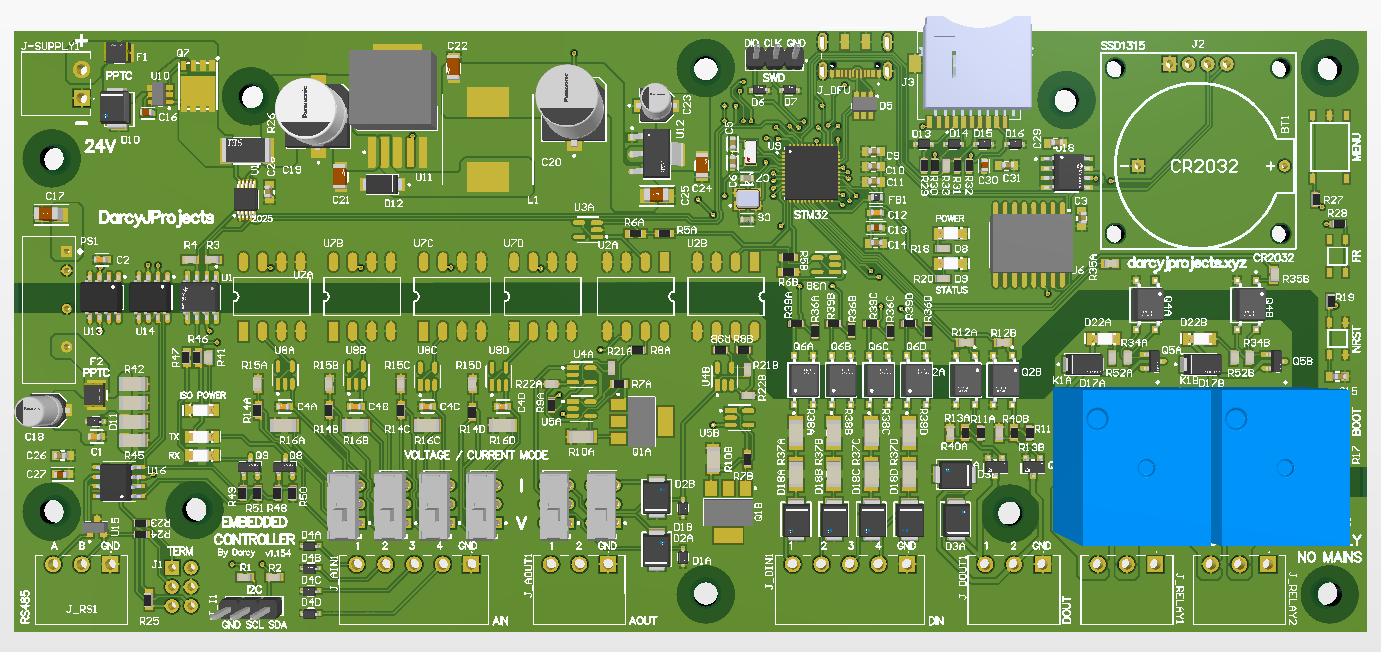
\includegraphics[width=.9\linewidth]{board_photo.png} 
    \caption{Board Top View}
\end{figure}


%\begin{figure}[h]
%    \centering
    % REPLACE 'example-image' with your block diagram
%    \includegraphics[width=0.8\linewidth]{example-image}
%    \caption{System Block Diagram}
%\end{figure}



% --- SECTION 2: DESCRIPTION ---
\section{General Description}
The \textbf{DJP-G431-EIC} is a robust embedded controller designed for industrial environments, bridging the gap between low-level microcontroller flexibility and PLC reliability. Built around the high-performance STM32G4 series, it features a high-efficiency 24V buck converter and \textbf{full galvanic isolation} on all field interfaces, ensuring system stability in noisy environments.

Unique to this controller is a \textbf{Hybrid Master-Slave} configuration handled by a custom \textbf{DMA-driven MODBUS RTU stack}. This allows the board to autonomously control downstream devices while simultaneously reporting to an upstream SCADA system or Web Panel. An on-board OLED display with burn-in protection provides local feedback on system status and configuration.

For logic control, the board natively supports a custom \textbf{Rule-Based Automation Engine}. This system is fully programmable over MODBUS using the Node.js Web Panel or manually with the vendor-defined functions, allowing for remote "No-Code" logic configuration without the need to reflash firmware.



% The "Research Purpose" Qualifier
\vspace{1em}
\begin{center}
\fbox{\parbox{0.95\linewidth}{
    \centering
    \scriptsize
    \textit{\textbf{DISCLAIMER:} This hardware is a personal engineering project created solely for \textbf{educational purposes and skill development}. While it explores industrial design techniques, it has \textbf{not} been tested against or certified for any specific industrial standards (e.g., IEC, UL, CE). It is provided "AS IS" without warranty.}
    
    \vspace{0.3em} % Tiny gap
    \textit{For full licence details, design files, and terms of use, please refer to the project repository at \textbf{github.com/DarcyJProjects}.}
}}
\end{center}


% Switch to single column for the big data tables
\onecolumn
\clearpage
\raggedbottom

\section{System Architecture}
The internal architecture of the DJP-G431-EIC is divided into two galvanically isolated domains: the \textbf{Logic Domain} (MCU, Main Power Supply, etc.) and the \textbf{Field Domain} (Field I/O, RS485, etc.). 

The following block diagram illustrates the power distribution path, isolation barriers, and internal peripheral connections. A physical separation width is maintained along the isolation barrier on the PCB utilising different electrical isolation methods (capacitive, optical, etc.), depending on the signal.

% BLOCK DIAGRAM
\begin{figure}[H]
    \centering
    % Reduced width slightly to 0.85 to ensure everything fits
    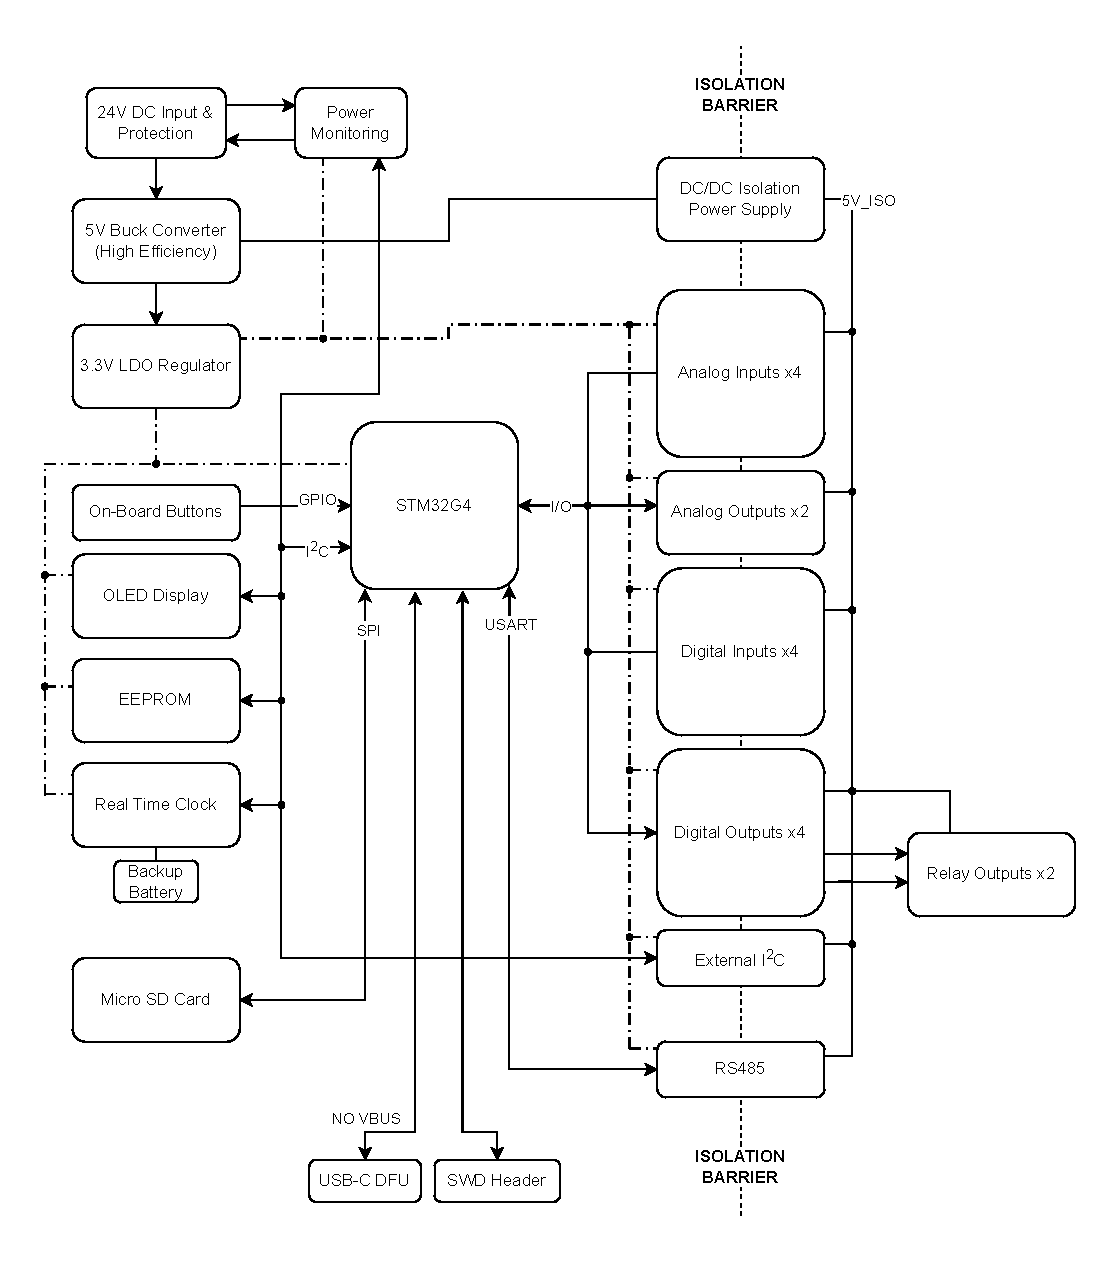
\includegraphics[width=0.85\linewidth]{general_block_diagram} 
    \caption{System Block Diagram showing Power Architecture and Galvanic Isolation.}
    \label{fig:general_block_diagram}
\end{figure}


\section{Electrical Specifications}
Conditions: $V_{IN} = 24V$, $T_A = 25^{\circ}C$ unless otherwise noted.


\begin{table}[H]
\caption{Isolation \& Protection Characteristics}
\begin{tabularx}{\textwidth}{l | c | c | X}
    \thickhline
    \textbf{Parameter} & \textbf{Symbol} & \textbf{Value} & \textbf{Conditions} \\
    \hline
    \multicolumn{4}{l}{\textit{\textbf{Galvanic Isolation}}} \\
    \hline
    \textbf{System Isolation} & $V_{ISO\_SYS}$ & \textbf{1000 VDC} & \textbf{Limited by DC/DC Power Supply} \\
    Data Channel Rating & $V_{ISO\_DAT}$ & 3750 Vrms & Component Rating (Isolators Only) \\
    Isolation Capacitance & $C_{ISO}$ & $\sim$40 pF & Barrier Capacitance (Typical) \\
    \hline
    \multicolumn{4}{l}{\textit{\textbf{ESD Protection}}} \\
    \hline
    \textbf{General I/O \& Power} & $V_{ESD\_GEN}$ & $\pm$30 kV & \textbf{IEC 61000-4-2} (Air \& Contact) \\
    \multicolumn{4}{l}{\textit{\footnotesize (Includes: Power In, Digital I/O, Analog I/O, SD Card, SWD)}} \\
    \hline
    \textbf{Comm. Interfaces} & $V_{ESD\_COM}$ & $\pm$15 kV & \textbf{IEC 61000-4-2} (Air) \\
     & & $\pm$8 kV & \textbf{IEC 61000-4-2} (Contact) \\
    \multicolumn{4}{l}{\textit{\footnotesize (Includes: RS485, USB DFU)}} \\
    \hline
    \textbf{I2C Expansion} & $V_{ESD\_I2C}$ & $\pm$4 kV & \textbf{HBM} (ISO1540 Native Rating) \\
    \hline
    \multicolumn{4}{l}{\textit{\textbf{EFT Immunity}}} \\
    \hline
    Power \& Field I/O & $V_{EFT}$ & 4 kV & \textbf{IEC 61000-4-4} (Level 4) \\
    \thickhline
\end{tabularx}
\end{table}


\begin{table}[H]
\caption{Over-Current Protection (PPTC Resettable Fuses)}
\begin{tabularx}{\textwidth}{l | c | c | c | X}
    \thickhline
    \textbf{Protected Rail} & \textbf{Hold} ($I_{HOLD}$) & \textbf{Trip} ($I_{TRIP}$) & \textbf{Max V} & \textbf{Notes} \\
    \hline
    Main Power Input ($V_{IN}$) & XX mA & $\sim$2x the hold mA  & 30 V & Protects entire board \\
    5V\_ISO & XX mA & $\sim$2x the hold mA & 6 V & Protects B0505S isolated DC/DC \\
    \thickhline
\end{tabularx}
\begin{tablenotes}
\footnotesize
\item \textbf{Note:} Fuses are self-resetting. To reset a tripped fuse, remove the fault and cycle power for $>10$ seconds.
\end{tablenotes}
\end{table}

\begin{table}[h]
\begin{threeparttable}
\caption{DC Characteristics}
\begin{tabularx}{\textwidth}{l | c | c c c | c | X}
    \thickhline
    \textbf{Parameter} & \textbf{Symbol} & \textbf{Min.} & \textbf{Typ.} & \textbf{Max.} & \textbf{Unit} & \textbf{Comments} \\
    \hline
    \multicolumn{7}{l}{\textbf{Power Supply}} \\
    \hline
    Supply Voltage      & $V_{IN}$   & 7  & 24  & 28  & V  & Operating Range \\
    Supply Current      & $I_{IN}$   & -   & XX  & XX & mA & Idle vs. All Relays Active \\
    \hline
    \multicolumn{7}{l}{\textbf{Digital Inputs}} \\
    \hline
    Input Voltage High  & $V_{IH}$   & XX  & 24  & 28  & V  & Logic "1" Threshold \\
    Input Voltage Low   & $V_{IL}$   & XX  & 0   & XX   & V  & Logic "0" Threshold \\
    Input Current       & $I_{DIN}$  & -   & 11.4   & 14.9  & mA & @ 24V (Typ) / 28V (Max) \\
    \hline
    \multicolumn{7}{l}{\textbf{Digital Outputs}} \\
    \hline
    Cont. Sink Current  & $I_{DOUT}$ & -   & -   & 500 & mA & \textbf{Sinking} Per Channel \\
    Output Voltage Drop & $V_{DROP}$ & -   & 10 & 16 & mV  & @ 500mA Load \\
    \hline
    \multicolumn{7}{l}{\textbf{Digital Outputs (Relays)}} \\
    \hline
    Switching Voltage (DC)   & $V_{SW}$   & -   & 24  & 30 & V  & DC Voltage  \\
    Switching Voltage (AC)   & $V_{SW}$   & -   & 24  & 50 & VAC  & AC Voltage  \\
    Switching Current   & $I_{SW}$   & -   & -   & 10  & A  & Max Resistive Load \\
    Contact Resistance  & $R_{CONT}$ & -   & - & 100   & m$\Omega$ & Initial value \\
    \hline
    \multicolumn{7}{l}{\textbf{Analog Inputs (12-Bit)}} \\
    \hline
    Input Impedance (V) & $R_{IN(V)}$& - & 49   & -   & k$\Omega$ & 0-5V Mode \\
    Input Impedance (I) & $R_{IN(I)}$& -   & 10 & -   & $\Omega$ & 4-20mA Mode \\
    \hline
    \multicolumn{7}{l}{\textbf{Analog Outputs (12-Bit)}} \\
    \hline
    Output Voltage      & $V_{OUT}$  & 0   & -   & 5   & V  & 0-5V Mode -- \textbf{Sourcing} (Active) \\
    Source Current      & $I_{SRC}$  & -   & -   & XX  & mA & 0-5V Mode -- Max drive \\
    \hline
    Current Sink Range\tnote{1}  & $I_{SNK}$  & X   & -   & XX  & mA & 4-20mA Mode -- \textbf{Sinking} (Passive) \\
    Max Loop Voltage\tnote{3}    & $V_{LOOP}$ & 12  & 24  & 30  & V  & 4-20mA Mode -- Ext. Loop Supply \\
    Max Loop Resistance & $R_{LOOP}$ & 300 & 900 & 1075 & $\Omega$ & @ 12V / 24V / 30V Loop Voltage \\
    \hline
    \multicolumn{7}{l}{\textbf{RS485 Interface}} \\
    \hline
    Bus Voltage Range\tnote{2}   & $V_{BUS}$  & -7  & -   & 12  & V  & Common Mode Range (A/B) \\
    Input Impedance     & $R_{IN}$   & 12  & -   & -   & k$\Omega$ & 1 Unit Load (Max 32 Nodes) \\
    \hline
    \multicolumn{7}{l}{\textbf{External $I^2C$ Expansion Header}} \\
    \hline
    Field Signal Voltages\tnote{2}      & $V_{SDA2}, V_{SCL2}$  & 0 & - & 5.0 & V  & Field Signal Voltages \\
    Pull-Up Resistance  & $R_{PU}$   & 4.4   & 4.7 & 5.0   & k$\Omega$ & On-Board $I^2C$ Field Pull-ups \\
    \thickhline
\end{tabularx}
\begin{tablenotes}
\footnotesize
% The \tnote{1} connects to the superscript 1 in the table
\item[1] \textbf{Note:} The exact 4mA and 20mA setpoints are determined by firmware calibration values. Improper configuration may result in output currents deviating from these nominal targets (e.g. $<4$mA or $>20$mA).
\item[2] Relative to 5V\_ISO\_GND (the GND pin in the field header or connector).
\item[3] \textbf{Important:} The maximum loop voltage drops significantly as the ambient temperature rises. See Absolute Maximum Ratings.
\end{tablenotes}
\end{threeparttable}
\end{table}

\clearpage


\section{Absolute Maximum Ratings}
\begin{table}[H]
\caption{Stress Ratings CALC CONFIRMED}
\begin{tabularx}{\textwidth}{l | c | c c | c | X}
    \thickhline
    \textbf{Parameter} & \textbf{Symbol} & \textbf{Min.} & \textbf{Max.} & \textbf{Unit} & \textbf{Comments} \\
    \hline
    \multicolumn{6}{l}{\textbf{Power}} \\
    \hline
    Input Voltage       & $V_{IN\_MAX}$  & - & 30 & V & Continuous (Limited by Input PPTC \& TVS) \\
    Max Total Current   & $I_{IN\_MAX}$  & - & XX & A & Limited by Input PPTC \\
    \hline
    \multicolumn{6}{l}{\textbf{Digital I/O}} \\
    \hline
    DIN Voltage         & $V_{DIN\_MAX}$ & - & 30 & V & Continuous (Thermal Limit of Series Resistors)\\
    \hline
    DOUT Sink Current   & $I_{DOUT\_MAX}$ & - & 3 & A & Continuous (Per Channel) @ $T_A = 85^{\circ}C$\\
    Relay Voltage       & $V_{SW\_MAX(DC)}$ & - & 110 & V & Max DC Contact Switching Voltage \\
    Relay Voltage       & $V_{SW\_MAX(AC)}$ & -  & 50 & VAC & Max AC Contact Switching Voltage \\
    Relay Current       & $I_{REL\_MAX}$ & - & 10 & A & Resistive Load \\
    \hline
    \multicolumn{6}{l}{\textbf{Analog I/O}} \\
    \hline
    AIN Voltage (V-Mode)& $V_{AIN\_MAX(V)}$ & -   & \textbf{5.5} & V & \textbf{Risk of Damage!} (Do not connect 24V) | Continuous (Limited by Input TVS)\\
    AIN Current (I-Mode)& $I_{AIN\_MAX(I)}$ & -   & 140 & mA & Max Loop Current (Shunt Resistor Limit) \\
    \hline
    AOUT Voltage (V-Mode)& $V_{AOUT\_MAX(V)}$ & - & \textbf{5.3} & V & \textbf{Risk of Damage!} (Do not connect 24V) | Max External Voltage applied to pin \\
    AOUT Voltage (I-Mode)& $V_{AOUT\_MAX(I)}$ & - & 26 & V & Max External Loop Voltage (Open Collector) @ $T_A = 85^{\circ}C$ \\
    \hline
    \multicolumn{6}{l}{\textbf{Communication Interfaces}} \\
    \hline
    RS485 Bus Voltage In   & $V_{485\_IN\_ABS}$ & -8 & +12.5 & V & Max voltage on A/B pins before damage \\
    RS485 Bus Voltage Out   & $V_{485\_OUT\_ABS}$ & -8 & +12.5 & V & Max voltage from driver to A/B pins \\
    I2C Pin Voltage     & $V_{I2C\_ABS}$ & -0.5 & 5.5 & V & Max voltages on SDA/SCL \\
    \hline
    \multicolumn{6}{l}{\textbf{Environmental}} \\
    \hline
    Storage Temp.       & $T_{STG}$      & -XX & +XX & $^{\circ}$C & Estimation\\
    Operating Temp.     & $T_{OP}$       & -XX & +XX & $^{\circ}$C & Estimation \\
    \thickhline
\end{tabularx}
\end{table}



\clearpage

\section{MODBUS Register Map}
% \vspace{-4em} % Pulls the table up by one line height
\begin{table}[H]
\small
\begin{threeparttable}
\caption{Complete Register Map}
\begin{tabularx}{\textwidth}{c | l | c | c | X}
    \thickhline
    \textbf{Addr} & \textbf{Name} & \textbf{Type} & \textbf{Access} & \textbf{Description} \\
    \hline
    \multicolumn{5}{l}{\textit{\textbf{Discrete Inputs (Digital Inputs)}}} \\
    \hline
    0 & DIN\_1 & Bool & R & Digital Input Channel 1 \\
    1 & DIN\_2 & Bool & R & Digital Input Channel 2 \\
    2 & DIN\_3 & Bool & R & Digital Input Channel 3 \\
    3 & DIN\_4 & Bool & R & Digital Input Channel 4 \\
    \hline
    \multicolumn{5}{l}{\textit{\textbf{Coils (Digital Outputs \& Relays)}}} \\
    \hline
    0 & DOUT\_1 & Bool & R/W & Digital Output 1 \\
    1 & DOUT\_2 & Bool & R/W & Digital Output 2 \\
    2 & RELAY\_1 & Bool & R/W & Relay Output 1 \\
    3 & RELAY\_2 & Bool & R/W & Relay Output 2 \\
    \hline
    \multicolumn{5}{l}{\textit{\textbf{Input Registers (Analog Inputs)}}} \\
    \hline
    0 & AIN\_1 & uint16 & R & Analog Input 1 Raw Value \\
    1 & AIN\_2 & uint16 & R & Analog Input 2 Raw Value \\
    2 & AIN\_3 & uint16 & R & Analog Input 3 Raw Value \\
    3 & AIN\_4 & uint16 & R & Analog Input 4 Raw Value \\
    \hline
    \multicolumn{5}{l}{\textit{\textbf{Holding Registers (Analog Outputs)}}} \\
    \hline
    0 & AOUT\_1 & uint16 & R/W & Analog Output 1 Setpoint (0-65535) \\
    1 & AOUT\_2 & uint16 & R/W & Analog Output 2 Setpoint (0-65535) \\
    \thickhline
\end{tabularx}
\begin{tablenotes}
\footnotesize
\item \textbf{Access Key:} R = Read Only, R/W = Read/Write. 
\item \textbf{Function Codes:} Discrete (0x02), Coils (0x01/0x05/0x15), Inputs (0x04), Holding (0x03/0x06/0x16).
\end{tablenotes}
\end{threeparttable}
\end{table}

\subsection{Virtual Registers}
Virtual Registers can be created dynamically to serve as intermediate variables within the automation logic (e.g., linking rules where the 2-condition limit per rule is exceeded).
\begin{itemize}
    \item \textbf{Addressing:} Virtual registers are automatically mapped starting at the address \textit{after} the last physical channel.
    \item \textit{Example:} If the last physical coil is Address 3, the first Virtual Coil will be \textbf{Address 4}.
\end{itemize}

Since Virtual Registers are defined with specific Modbus data types, they can be fully accessed (Read/Write) using standard Modbus function codes.

\subsection{External Expansion ($I^2C$)}
The isolated 5V $I^2C$ header allows external peripherals to be mapped to MODBUS registers. On-board field side 5V\_ISO pull-up resistors (4.7 k$\Omega$) are installed on SCL and SDA, so 5V tolerant $I^2C$ devices can only be used without an external level shifter (see Texas Instruments PCA9306). The user must provide their own power supply for the devices, and reference this to the GND pin in the header.
\vspace{1em} \\
\textit{\textbf{Note:} Unlike the Rule Engine, adding new $I^2C$ devices requires custom read/write drivers and a \textbf{firmware update}. Reference implementations for common sensors can be found in the project source code.}


\clearpage
\subsection{Vendor Defined Function Codes}
These proprietary function codes provide access to specialized device capabilities, including the internal logic engine and virtual register management, that are not covered by standard MODBUS definitions.
\textbf{Range:} 0x65--0x73 (Firmware Defined)
\begin{table}[H]
\begin{tabularx}{\textwidth}{c | l | X}
    \thickhline
    \textbf{Code} & \textbf{Name} & \textbf{Description} \\
    \hline
    0x65 & ADD\_RULE & Defines a new automation rule \\
    0x66 & GET\_RULE\_COUNT & Returns the number of automation rules \\
    0x67 & GET\_RULE & Returns the requested automation rule configuration \\
    0x68 & DELETE\_RULE & Deletes the requested automation rule \\
    0x69 & ADD\_VIRTUAL\_REG & Defines a new virtual register \\
    0x6A & READ\_VIRTUAL\_REG & Returns the value of the requested virtual register \\
    0x6B & WRITE\_VIRTUAL\_REG & Write the specified value to the requested virtual register \\
    0x6C & GET\_VIRTUAL\_REG\_COUNT & Returns the number of virtual registers \\
    0x6D & CLEAR\_VIRTUAL\_REG & Deletes all virtual registers. Warning: Do no execute if there are \textbf{any} rules that reference \textbf{any} virtual registers. \\
    0x6E & SET\_RTC & Sets the RTC date and time \\
    0x6F & SET\_HOLDING\_REG\_MODE & Sets the requested virtual register to the specified mode (current/voltage) \\
    0x70 & SET\_INPUT\_REG\_MODE & Sets the requested input register to the specified mode (current/voltage) \\
    0x71 & GET\_REG\_MODE & Returns the mode (current/voltage) of the requested register (holding/input) \\
    0x72 & SET\_EMERGENCY\_STOP & Sets the E-STOP button configuration \\
    0x73 & FACTORY\_RESET & Performs a factory reset, resetting the on-board EEPROM to default values \\
    \thickhline
\end{tabularx}
\end{table}

\textbf{Note:} Function codes 0x6F--0x73 extend into the Public Function Code range. 
While functionally valid for this device, they are non-standard. Future firmware revisions 
may migrate all vendor-defined functions into a Sub-Function Encapsulation architecture (e.g. Function Code 0x64).

\section{Software Ecosystem}
The DJP-G431-EIC is supported by a comprehensive software suite:
\begin{itemize}
    \item \textbf{Web Configuration Panel:} A Node.js-based dashboard connecting via the USB-Serial bridge. Allows for real-time monitoring of all registers, hardware configuration, and "No-Code" logic automation; all over MODBUS RTU.
    \item \textbf{Automation Engine:} Custom logic engine supporting drop-down based "If-This-Then-That" rules, executed locally on the STM32, programmed over MODBUS vendor functions.
\end{itemize}

\clearpage

\section{User Interface}

\subsection{Button Functions}
The board features 4 tactile buttons for menu interaction, system recovery, and boot control.

\begin{table}[h]
\begin{tabularx}{\textwidth}{l | l | X}
    \thickhline
    \textbf{Button} & \textbf{Function} & \textbf{Description} \\
    \hline
    \textbf{MENU} & Navigation & Short Press: Next Menu Screen \\
    \textbf{NRST} & System Reset & Short Press: Hardware Reset (Reboots MCU) \\
    \hline
    \textbf{BOOT0 + NRST} & DFU Mode & Hold BOOT0 and short press NRST to enter DFU mode. OLED should indicate that DFU mode has been entered. \\
    \textbf{FR + NRST} & Factory Reset & Hold FR and short press NRST to restore default configuration options on the EEPROM. Further button press instructions will be provided on the OLED. \\
    \textbf{MENU + NRST} & Skip Boot Animations & Hold MENU and short press NRST to skip boot animations when starting. Useful for quick tests during firmware development. \\
     \thickhline
\end{tabularx}
\end{table}

\subsection{LED Indicators}
\begin{table}[H]
\begin{tabularx}{\textwidth}{l | c | X}
    \thickhline
    \textbf{Name} & \textbf{Color} & \textbf{Indication} \\
    \hline
    \textbf{PWR} & Green & 3.3V Logic Domain Power Active \\
    \textbf{ISO\_PWR} & Green & 5V Isolated Field Domain Power Active \\
    \textbf{RX/TX} & Blue & Modbus RS485 Data Traffic \\
    \textbf{REL1 / REL2} & Yellow & Relay Coil Energized (Output Active) \\
    \thickhline
\end{tabularx}
\end{table}


\subsection{RS485 Bus Configuration}
The isolated RS485 interface features a 6-pin jumper header (JP\_RS485) to enable line termination and failsafe biasing. These should be configured based on the device's position in the network.

\vspace{0.5em}

\noindent
\begin{minipage}{0.35\textwidth}
    \centering
    \textbf{Jumper Map (Top View)} \\
    \vspace{0.5em}
    % This grid mimics the physical 2x3 header on your PCB
    \begin{tabular}{|c|c|}
        \hline
        \footnotesize \textbf{1} (A) & \footnotesize \textbf{2} (PULL\_UP) \\
        \hline
        \footnotesize \textbf{3} (B) & \footnotesize \textbf{4} (PULL\_DOWN) \\
        \hline
        \footnotesize \textbf{5} (A) & \footnotesize \textbf{6} (TERM. TO B) \\
        \hline
    \end{tabular}
    \\ \vspace{0.5em}
    \footnotesize \textit{Bridge adjacent pins to enable.}
\end{minipage}%
\hfill
\begin{minipage}{0.6\textwidth}
    \textbf{Configuration Settings:}
    \begin{itemize}[noitemsep, leftmargin=1.5em, topsep=0pt]
        \item \textbf{Bias High (Pins 1-2):} Pulls Line A to 5V\_ISO. \textit{Keeps bus logic "1" during idle.}
        \item \textbf{Bias Low (Pins 3-4):} Pulls Line B to 5V\_ISO\_GND. \textit{Keeps bus logic "0" during idle.}
        \item \textbf{Termination (Pins 5-6):} Connects a $120\Omega$ resistor across lines A and B. \textit{Enable only if this device is at the physical end of the bus cable.}
    \end{itemize}
\end{minipage}

\vspace{0.5em}
\noindent \textit{\footnotesize \textbf{Note:} Failsafe biasing (Pins 1-4) is recommended to prevent noise interpretation when the bus is idle, but ensure only ONE device on the bus provides biasing (usually the Master).}


\clearpage
\section{Mechanical \& Installation}

\begin{figure}[h]
    \centering
    % REPLACE with your Mechanical Drawing (PCB Outline + Hole Dimensions)
    % \includegraphics[width=0.7\linewidth]{mechanical_drawing} 
    \begin{center}
        \fbox{\parbox{10cm}{\centering \vspace{3cm} [PLACEHOLDER: PCB DIMENSIONS \& MOUNTING HOLES] \vspace{3cm}}}
    \end{center}
    \caption{Mechanical Dimensions (Units: mm). Mounting Holes are M3 standard.}
\end{figure}

\section{Connection Diagram}
\begin{figure}[H]
    \centering
    % REPLACE with your "Coloured Wires" diagram
    % \includegraphics[width=0.9\linewidth]{wiring_diagram}
    \begin{center}
        \fbox{\parbox{12cm}{\centering \vspace{4cm} [PLACEHOLDER: SENSOR \& ACTUATOR WIRING DIAGRAM] \vspace{4cm}}}
    \end{center}
    \caption{Typical Connection Example. Note: Analog I/O must be configured via slide switches before powering on, and via the web panel or vendor-defined functions post-boot. }
\end{figure}



%\vfill % Pushes this to the bottom of the page

%\begin{center}
%\fbox{\parbox{0.9\textwidth}{
%    \centering
%    \scriptsize
%    \textit{\textbf{DISCLAIMER:} This hardware is a personal engineering project created solely for \textbf{educational purposes and %skill development}. While it explores industrial design techniques, it has \textbf{not} been tested against or certified for any specific %industrial standards (e.g., IEC, UL, CE). It is provided "AS IS" without warranty.}
%    
%    \vspace{0.3em} % Tiny gap
%    \textit{For full licence details, design files, and terms of use, please refer to the project repository at \textbf{github.com/%DarcyJProjects}.}
%}}
%\end{center}

\end{document}